%-------------------------
% Resume in Latex
% Author : Yauheni Baltukha
% Based off of: https://github.com/baltuky/latex-cv
% License : MIT
%------------------------

\documentclass[a4, 11pt]{article}

\usepackage{latexsym}
\usepackage[empty]{fullpage}
\usepackage{titlesec}
\usepackage{marvosym}
\usepackage[usenames, dvipsnames]{color}
\usepackage{verbatim}
\usepackage{enumitem}
\usepackage[hidelinks]{hyperref}
\usepackage{fancyhdr}
\usepackage[english]{babel}
\usepackage{tabularx}
\usepackage{ragged2e}
\usepackage{fontawesome}
\usepackage{graphicx}
\usepackage[absolute,overlay]{textpos}
\usepackage{amsmath}
\input{glyphtounicode}

%----------FONT OPTIONS----------
% sans-serif
\usepackage[sfdefault]{FiraSans}
\usepackage[sfdefault]{roboto}
\usepackage[sfdefault]{noto-sans}
\usepackage[default]{sourcesanspro}

% serif
% \usepackage{CormorantGaramond}
% \usepackage{charter}

\pagestyle{fancy}
\fancyhf{} % clear all header and footer fields
\fancyfoot{}
\renewcommand{\headrulewidth}{0pt}
\renewcommand{\footrulewidth}{0pt}

% Adjust margins
\addtolength{\oddsidemargin}{-0.5in}
\addtolength{\evensidemargin}{-0.5in}
\addtolength{\textwidth}{1.0in}
\addtolength{\topmargin}{-0.5in}
\addtolength{\textheight}{0.8in}

\urlstyle{same}

\raggedbottom
\raggedright
\setlength{\tabcolsep}{0in}

% Sections formatting
\titleformat{\section}{ \vspace{-4pt}\scshape\raggedright\large }{}{0em}{}[
\color{black}
\titlerule
\vspace{-5pt}
]

% Ensure that generate pdf is machine readable/ATS parsable
%\pdfgentounicode=1

%-------------------------
% Custom commands
\newcommand{\resumeItem}[1]{ \item\small{ {#1 \vspace{-2pt}} } }

\newcommand{\resumeSubheading}[4]{
\vspace{-2pt}
\item
\begin{tabular*}{0.97\textwidth}[t]{l@{\extracolsep{\fill}}r}
	\textbf{#1}       & #2                 \\
	\textit{\small#3} & \textit{\small #4} \\
\end{tabular*}
\vspace{-7pt}}

\newcommand{\resumeSubSubheading}[2]{ \item
\begin{tabular*}{0.97\textwidth}{l@{\extracolsep{\fill}}r}
	\textit{\small#1} & \textit{\small #2} \\
\end{tabular*}
\vspace{-7pt}
}

\newcommand{\resumeProjectHeading}[2]{ \item
\begin{tabular*}{0.97\textwidth}{l@{\extracolsep{\fill}}r}
	\small#1 & #2 \\
\end{tabular*}
\vspace{-7pt}
}

\newcommand{\resumeSubItem}[1]{\resumeItem{#1}
\vspace{-4pt}}

\renewcommand{\labelitemii}{$\vcenter{\hbox{\tiny$\bullet$}}$}

\newcommand{\resumeSubHeadingListStart}{\begin{itemize}[leftmargin=0.15in, label={}]}
\newcommand{\resumeSubHeadingListEnd}{\end{itemize}}
\newcommand{\resumeItemListStart}{\begin{itemize}}
\newcommand{\resumeItemListEnd}{\end{itemize}
\vspace{-5pt}}

%-------------------------------------------
%%%%%%  RESUME STARTS HERE  %%%%%%%%%%%%%%%%%%%%%%%%%%%%
\begin{document}
	%----------HEADING----------
 
	\begin{center}
		\textbf{\Huge \scshape Shafin Ahmed} \\
		\vspace{1pt}
		\small A versatile software engineer with 4 years of experience
	\end{center}

        % \begin{textblock}{3}(14.0,0.2) % Adjust the position here
        % 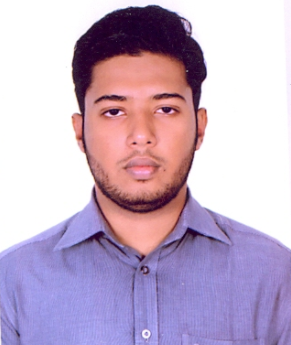
\includegraphics[width=0.5\linewidth]{Shafin Ahmed.png} % Adjust width to desired image size
        % \end{textblock}

	\begin{center}
		\raisebox{-0.2\height}{\Large \faPhoneSquare} \ \ \href{tel:+8801711382280}{+8801711382280}
		\hfill\raisebox{-0.2\height}{\Large \faEnvelopeSquare} \ \ \href{mailto:shafinwork580@gmail.com}{shafinwork580@gmail.com}
		\hfill \raisebox{-0.2\height}{\Large \faLinkedinSquare} \ \ \href{https://www.linkedin.com/in/shafin580/}{shafin580}
		\hfill\raisebox{-0.2\height}{\Large \faGithubSquare} \ \ \href{https://github.com/Shafin580}{Shafin580} \hfill\raisebox{-0.2\height}{\Large
		\faGlobe}
		\ \ \href{https://portfolio-shafin580s-projects.vercel.app/}{portfolio site}
	\end{center}

	%-----------SUMMARY-----------
	% \section{Summary}
	% \justify
	% With over a decade of experience as a software engineer, I have successfully contributed to both small and large-scale
	% companies. As a versatile engineer, my true passion lies in constructing robust and scalable systems,
	% specializing in the development of backend services and data pipelines.
	% My enthusiasm for problem-solving and the inherent joy I find in overcoming intricate engineering challenges fuel my
	% drive to build innovative solutions.

	%-----------EXPERIENCE-----------
	\section{Experience}
	\resumeSubHeadingListStart

    \resumeSubheading {Software Engineer}{Present} {ARITS Limited}{Baridhara DOHS, Dhaka}
	\begin{description}
		\item[] {\small\setlength{\baselineskip}{0.8\baselineskip} Spearheaded the development of sophisticated, responsive user interfaces, integrating advanced features like real-time data synchronization, global state management, and multi-factor authentication. Collaborated with backend developers, planning and building system architecture. implementing Tanstack Query for seamless database interactions, leading to improved data consistency and query performance. Integrated Stripe payment gateway into various projects. Implemented notification and messeging services on the frontend. Helped developing microservices for modular architecture, applying encryption techniques for secure data transactions. Streamlined deployment workflows by containerizing applications with Docker, achieving a 50\% reduction in deployment time.}
	\end{description}
 
	\resumeSubheading {Junior Software Engineer}{Sept 2022 -- June 2024} {ARITS Limited}{Baridhara DOHS, Dhaka}
	\begin{description}
		\item[] {\small\setlength{\baselineskip}{0.8\baselineskip} Designed over a dozen of complex and responsive UIs, implementing advanced features like global state management and authentication systems. Built multiple Frontend reusable components using Next.js, applied cryptography for data security. Containerized applications with Docker, enhancing full-stack development capabilities for over 40\% of deployments.}
	\end{description}

	\resumeSubheading {Internship Trainee}{June 2022 - Sept 2022} {ARITS Limited}{Baridhara DOHS, Dhaka}
	\begin{description}
		\item[] {\small\setlength{\baselineskip}{0.8\baselineskip} Developed web applications with Next.js, emphasizing server-side rendering and crafting engaging user interfaces using versatile animation libraries. Gained hands-on experience in building and integrating RESTful API endpoints while managing data fetching and state with modern front-end libraries. Additionally, developed backend services and REST APIs using Laravel, integrating Elasticsearch for optimized data querying and retrieval.}
	\end{description}

	\resumeSubHeadingListEnd

 %-----------PROGRAMMING SKILLS-----------
	\section{Technical Skills}
	\begin{itemize}[leftmargin=0.15in, label={}]
		\item{ 
            \textbf{Languages}{: Javascript, Typescript, PHP, Python, Java, C, C++, C\#, HTML, CSS}
        } 

        \item{ 
            \textbf{Databases}{: MySql, Postgresql, MongoDB, Elasticsearch, GraphQL}
        }
        
        \item{ 
            \textbf{Framework \& Library}{: Laravel, NextJS, ReactJS, Tailwindcss, Django, NestJS, NodeJS}
        }
        
        \item{ 
            \textbf{Technologies}{: JIRA, Git, Docker, Turborepo, Headless Wordpress, Zustand, Redux, Context API, TanStack Query, Puppeteer, Electron}
        }
	\end{itemize}

	%-----------PROJECTS-----------
	\section{Projects}
	\resumeSubHeadingListStart

    \resumeProjectHeading
      {\textbf{HRMS (In-house Product)} $|$ \emph{Next.js 16 | Typescript | Cryptography | Tanstack | Tailwindcss | ShadCN | TurboRepo}}
      {Present}
      \resumeItemListStart 
        \resumeItem{\textbf{Frontend Development:} Architected and developed the frontend codebase for an HRMS web app using Next.js 16, implementing best practices for scalable and maintainable code structure.}
        \resumeItem{\textbf{Single Sign-On (SSO):} Designed a secure login flow with middleware to share encrypted cookies across subdomains, enabling seamless user authentication across multiple modules without repeated logins, redirecting invalid users to the main module’s login page.}
        \resumeItem{\textbf{Optimized Codebase with Turborepo:} Utilized Turborepo to create and publish shared packages for common functions, reducing code duplication and enhancing maintainability across the project.}
        \resumeItem{\textbf{API Integration:} Spearheaded API consumption using TanStack Query, ensuring efficient data fetching and state management across the application.}
        \resumeItem{\textbf{Enhanced Security:} Implemented cookie encryption to secure user data and maintain session integrity across subdomains.}
        \resumeItem{\textbf{Developed Custom Components:} Built reusable and dynamic UI components, including a \href{https://dynamic-form-builder-ruddy.vercel.app/}{Dynamic Form Builder}, \href{https://routine-builder-app.vercel.app/}{Weekly Routine Builder}, \href{https://routine-calendar-app.vercel.app/}{Custom Calendar Routine}, \href{https://attendance-app-two-beta.vercel.app/}{Attendance Clock In-Out}, and \href{https://attendance-summary-app-alpha.vercel.app/}{Attendance Report UI}, improving user experience and functionality.}
    \resumeItemListEnd

     \resumeProjectHeading {\textbf{\href{https://bullwip.aritsltd.com/}{Bullwip}} $|$ Fullstack $|$ \emph{Next.js 16 | Typescript | Docker | Shadcn | Tailwindcss | Laravel | Postgressql | Elasticsearch}}
	{
	{Present}
	} \resumeItemListStart 
        \resumeItem{\textbf{Fullstack Development:} Architected a full-stack rental onboarding platform using Next.js for a responsive frontend and Laravel for a robust backend API, specifically tailored to the UK housing market.}
        \resumeItem{\textbf{API Integration:} Spearheaded API consumption using TanStack Query, ensuring efficient data fetching and state management across the application.}
        \resumeItem{\textbf{Enhanced Security:} Implemented cookie encryption to secure user data and maintain session integrity across subdomains.}
	\resumeItemListEnd

    \resumeProjectHeading
      {\textbf{Datafast} $|$ Fullstack $|$ \emph{Laravel | MySql | Electron | Next.js 14 | Typescript | Puppeteer | Docker}}
      {Present}
      \resumeItemListStart 
        \resumeItem{\textbf{Data Normalization:} Enhanced data handling and performance with effective frontend normalization techniques.}
        \resumeItem{\textbf{Automation:} Integrated seamless web automation using Puppeteer for efficient browser-based task execution}
        \resumeItem{\textbf{Infrastructure:} Designed and developed the entire system from scratch, wrapping the application with Electron for seamless desktop deployment.}
        \resumeItem{\textbf{Design:} Implemented Tailwind CSS and ShadCN, enhancing UI consistency and development efficiency.}
\resumeItemListEnd

    \resumeProjectHeading
      {\textbf{\href{https://www.calternatives.org/}{calternatives.org}} $|$ Fullstack $|$ \emph{Headless Wordpress | GraphQL | ACF | SEO | Next.js 14 | Typescript | Docker | SSG | SSR}}
      {Jan 2025}
      \resumeItemListStart 
        \resumeItem{\textbf{Data Normalization:} Enhanced data handling and performance with effective frontend normalization techniques.}
        \resumeItem{\textbf{Headless WordPress Integration:} Integrated WordPress with GraphQL and ACF for flexible content management and efficient data retrieval, resulting 70\% increase in development speed}
        \resumeItem{\textbf{Technical SEO:} Applied sitemap, robots configuration and technical SEO best practices to boost visibility and search engine performance by 65\%}
        \resumeItem{\textbf{Design:} Implemented Tailwind CSS and ShadCN, enhancing UI consistency and development efficiency.}
\resumeItemListEnd

 %    \resumeProjectHeading
	% {\textbf{\href{https://betterbangladesh.io/}{betterbangladesh.io}} $|$ Front-end $|$ \emph{Next.js 14, TypeScript, Tanstack Query, API Consumption, Context API}}
	% {
 %        {Aug 2024}
	% } \resumeItemListStart 
 % \resumeItem{\textbf{UI Component Design:} Designed modular, responsive UI components, ensuring a cohesive user experience.}
	% \resumeItem{\textbf{API Integration:} Managed full API consumption, optimizing data flow and performance.}
 % \resumeItem{\textbf{Project Leadership:} Led project planning, team workflows, and development oversight to meet project goals on time.}
	% \resumeItemListEnd

    \resumeProjectHeading {\textbf{\href{https://www.arits.tech/}{arits.tech}} $|$ Fullstack $|$ \emph{Headless Wordpress | GraphQL | ACF | SEO | Webflow | Javascript | Docker}}
	{
	{Feb 2024}
	} \resumeItemListStart 
        \resumeItem{\textbf{Data Normalization:} Improved data management and performance by 30\% through frontend data
normalization.}
	\resumeItem{\textbf{Requirement Analysis \& Development:} Planned and developed project      requirements for clear objectives and efficient execution.}
        \resumeItem{\textbf{Headless WordPress Integration:} Integrated WordPress with GraphQL and ACF for flexible content management and efficient data retrieval, resulting 40\% increase in development speed}
        \resumeItem{\textbf{Technical SEO:} Applied sitemap, robots configuration and technical SEO best practices to boost visibility and search engine performance by 45\%}
	\resumeItemListEnd

	\resumeSubHeadingListEnd

	%-----------CERTIFICATION-----------
	\section{Certifications}
	\resumeSubHeadingListStart \resumeSubheading {Responsive Web Development, CodersTrust}{Dhaka, Bangladesh}
	{ }{Mar 2020} \resumeSubHeadingListEnd

	%-------------------------------------------
 
    %-----------EDUCATION-----------
	\section{Education}
	\resumeSubHeadingListStart \resumeSubheading {Computer Science and Engineering, American International University-Bangladesh }{Dhaka, Bangladesh}
	{Bachelor of Science -- 3.58/4}{Jan 2018 -- April 2022}
        {Thesis: Machine Learning: Train AI to detect sentiment in a sentence}
 \resumeSubHeadingListEnd

 %-----------REFERENCES-----------
\section{References}
\resumeSubHeadingListStart
    \item \textbf{\href{https://www.linkedin.com/in/mosabber-uddin-ahmed-53798b16/}{Mosabber Uddin Ahmed}}, Senior Project Manager, Exabyting \\
    Email: \href{mailto:bapon.bu@gmail.com}{bapon.bu@gmail.com} \\
    Phone: \href{tel:+8801780444466}{+8801780444466}
    \item \textbf{\href{https://www.linkedin.com/in/emranffl/}{Emran Hossain}}, Senior Software Engineer, Gain Solutions Ltd \\
    Email: \href{mailto:emranffl.biz@gmail.com}{emranffl.biz@gmail.com} \\
    Phone: \href{tel:+8801676987366}{+8801676987366}
\resumeSubHeadingListEnd

	%-------------------------------------------
\end{document}
